\title{%
  DD1301 Datorintroduktion
}
\author{Daniel Bosk}
\institute{%
  KTH EECS
}

\mode<article>{\maketitle}
\mode<presentation>{%
  \begin{frame}
    \maketitle
  \end{frame}
}

\mode*


\section{What to learn?}

\subsection{Terminal}

\begin{frame}
  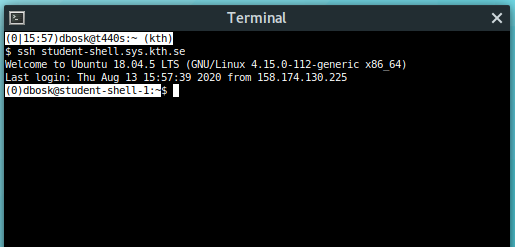
\includegraphics[width=\columnwidth]{../../terminal/terminal.png}
\end{frame}

\begin{frame}[fragile]
  \begin{lstlisting}[numbers=none]
n=10 cat hitch-hikers-guide.txt | \
  tr -cs A-Za-z '\n' | tr A-Z a-z | \
  sort | \
  uniq -c | \
  sort -rn | \
  head -n \$n
  \end{lstlisting}
\end{frame}


\subsection{Version management}

\begin{frame}
  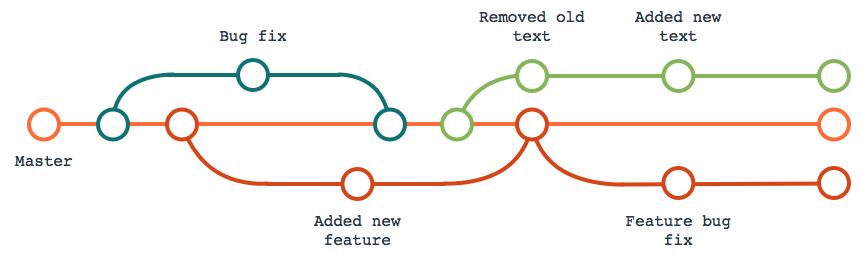
\includegraphics[width=\columnwidth]{version-tree.png}
\end{frame}


\subsection{\LaTeX}

\begin{frame}
\[
  f(x, y) = \sum_{i=1}^n 
  \frac{x^{\frac{2^{2^{2^{2^n}}}}{\sqrt{1-\frac{v^2}{c^2}}}}}{y}
\]

%  \begin{lstlisting}
%R^*=\argmin_{\substack{RR^t=I,\\ \det(R)=1}}
%    \sum_{i=1}^n \omega_i \norm{RX_i-Y_i}^2_2,
%  \end{lstlisting}
\end{frame}

\begin{frame}[fragile]
  \lstinputlisting[firstline=19,firstnumber=19,lastline=37]{contents.tex}
\end{frame}


\section{The course}

\subsection{Course material}

\begin{frame}
  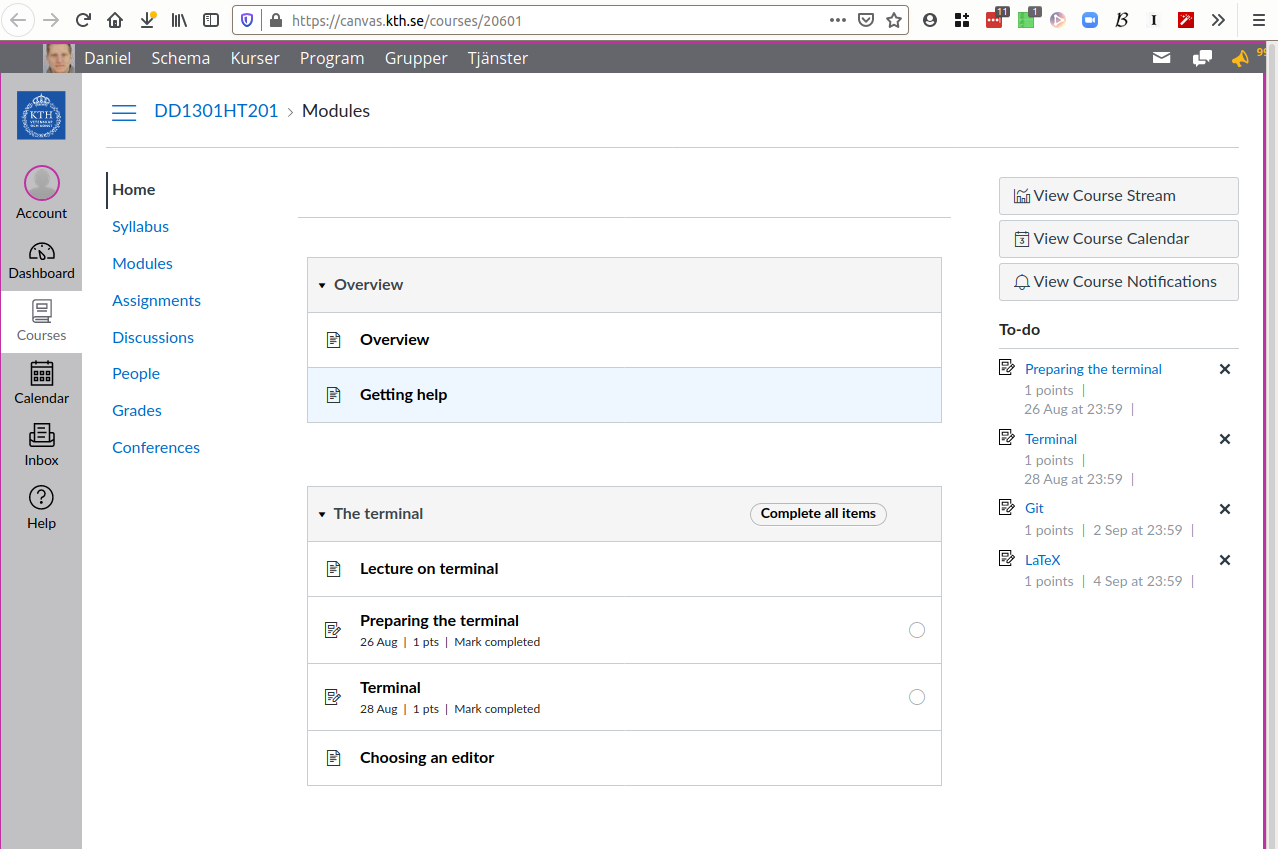
\includegraphics[width=\columnwidth]{canvas.png}
\end{frame}

\subsection{The labs}

\begin{frame}
  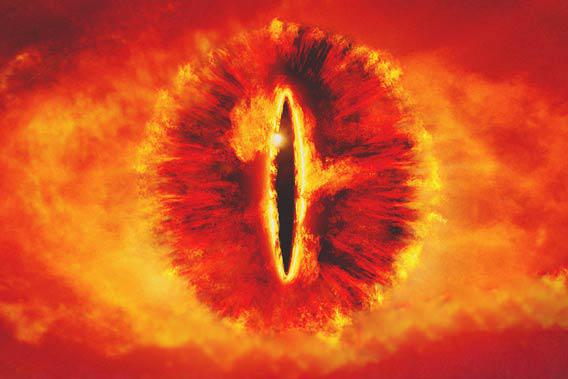
\includegraphics[width=\columnwidth]{sauron.jpg}
\end{frame}


%%% REFERENCES %%%

\begin{frame}[allowframebreaks]
  \printbibliography{}
\end{frame}
